\documentclass[11pt,a4paper,notitlepage]{article}

\usepackage[T1]{fontenc}
\usepackage[utf8]{inputenc}
\usepackage[english]{babel}
\usepackage{fullpage}
\usepackage{amsmath}
\usepackage{amsfonts}
\usepackage{amssymb}
\usepackage{verbatim}
\usepackage{listings}
\usepackage{color}
\usepackage{setspace}
\usepackage{epstopdf}
\usepackage{graphicx}
\usepackage{caption}
\usepackage{subcaption}
\usepackage{float}
\usepackage{epstopdf}
\usepackage{hyperref}
\usepackage{braket}
\pagenumbering{arabic}

\definecolor{codepurple}{rgb}{0.58,0,0.82}
\definecolor{backcolour}{rgb}{0.95,0.95,0.92}
\definecolor{dkgreen}{rgb}{0,0.6,0}
\definecolor{gray}{rgb}{0.5,0.5,0.5}
\definecolor{mauve}{rgb}{0.58,0,0.82}
%\setlength{\parindent}{0pt}

\lstdefinestyle{pystyle}{
  language=Python,
  aboveskip=3mm,
  belowskip=3mm,
  columns=flexible,
  basicstyle={\small\ttfamily},
  backgroundcolor=\color{backcolour},
  commentstyle=\color{dkgreen},
  keywordstyle=\color{magenta},
  numberstyle=\tiny\color{gray},
  stringstyle=\color{codepurple},
  basicstyle=\footnotesize,  
  breakatwhitespace=false
  breaklines=true,
  captionpos=b,
  keepspaces=true,
  numbers=left,
  numbersep=5pt,
  showspaces=false,
  showstringspaces=false,
  showtabs=false,
  tabsize=2
}
\lstdefinestyle{iStyle}{
  language=IDL,
  aboveskip=3mm,
  belowskip=3mm,
  columns=flexible,
  basicstyle={\small\ttfamily},
  backgroundcolor=\color{backcolour},
  commentstyle=\color{dkgreen},
  keywordstyle=\color{magenta},
  numberstyle=\tiny\color{gray},
  stringstyle=\color{codepurple},
  basicstyle=\footnotesize,  
  breakatwhitespace=false
  breaklines=true,
  captionpos=b,
  keepspaces=true,
  numbers=left,
  numbersep=5pt,
  showspaces=false,
  showstringspaces=false,
  showtabs=false,
  tabsize=2
}
\lstdefinestyle{c++style}{
  language=C++,
  keywordstyle=\color{blue}\ttfamily,
  stringstyle=\color{red}\ttfamily,
  commentstyle=\color{green}\ttfamily,
  morecomment=[l][\color{magenta}]{\#}
  aboveskip=3mm,
  belowskip=3mm,
  columns=flexible,
  basicstyle={\small\ttfamily},
  backgroundcolor=\color{backcolour},
  numberstyle=\tiny\color{gray},
  basicstyle=\footnotesize,  
  breakatwhitespace=false
  breaklines=true,
  captionpos=b,
  keepspaces=true,
  numbers=left,
  numbersep=5pt,
  showspaces=false,
  showstringspaces=false,
  showtabs=false,
  tabsize=2
}

\title{\normalsize Fys4150: Computational Physics \\
\vspace{10mm}
\huge Project 1\\
\vspace{10mm}
\normalsize Due date {\bf 19.th of September, 2016 - 23:59}}

% Skriv namnet ditt her og fjern kommenteringa
\author{Øyvind B. Svendsen, Magnus Christopher Bareid \\ un: oyvinbsv, magnucb}

\newcommand\pd[2]{\frac{\partial #1}{\partial #2}}
\def\doubleunderline#1{\underline{\underline{#1}}}


\begin{document}
\noindent
\maketitle
\vspace{10mm}
\begin{abstract}
The aim of this project is for the students to get familiar with various vector and matrix operations, from dynamic memory allocation to the usage of programs in the library package of the course.

The students were invited to use either brute force-algorithms to calculate linear algebra, or to use a set of recommended linear algebra packages, i.e. Armadillo, that simplify the syntax of linear algebra. Additionally, dynamic memory handling is expected.

The students will showcase necessary algebra to perform the tasks given to them, and explain the way said algebra is implemented into algorithms. In essence, we're asked to simplify a linear second-order differential equation from the form of the Poisson equation, seen as
\begin{align*}
\nabla ^2 \Phi = -4\pi\rho(\mathbf{r})
\end{align*}
into a one-dimensional form bounded by Dirichlet boundary conditions.
\begin{align*}
-u''(x) = f(x)
\end{align*}
so that discretized linear algebra may be committed unto the equation, yielding a number of numerical methods for aquiring the underivated function $u(x)$.
\end{abstract}
\begin{center}
\line(1,0){450}
\end{center}

%\newpage
\tableofcontents

\newpage
\section{Computational Physics, first project}
\subsection{The fundamental math}
\subsubsection{Introduction}
The production of this document will inevitably familiarize its authors with the programming language \verb|C++|, and to this end mathematical groundwork must first be elaborated to translate a Poisson equation from continuous calculus form, into a discretized numerical form.

The Poisson equation is rewritten to a simplified form, for which a real solution is given, with which we will compare our numerical approximation to the real solution.

The real motivation for this project, though, is to find a viable numerical method for double integration and the implementation of such.

\subsubsection{Problem}
%something something dark side about how we decompose the abstract problem into a real programmable problem

\section{Method}
\label{section:method}

Reviewing the Poisson equation:
\begin{align*}
\nabla ^2 \Phi &= -4\pi\rho(\mathbf{r}), \ \text{which is simplified one-dimensionally by} \ \Phi(r) = \phi(r)/r \\
\Rightarrow \frac{d^2 \phi}{dr^2} &= -4\pi r \rho(r), \ \text{which is further simplified by these substitutions:}\\
r &\rightarrow x, \\
\phi &\rightarrow u,\\
4\pi r\rho(r) &\rightarrow f, \indent \text{which produces the simplified form}
\end{align*}\begin{align*}\label{eq:1}\tag{1}
-u''(x) &= f(x), \indent \text{for which we assume that} \indent f(x) = 100e^{-10x}, \\
\Rightarrow u(x) &= 1- (1-e^{-10})x - e^{-10x},\ \text{with bounds:}\ x \in [0,1],\ u(0) = u(1)= 0
\end{align*}
From here on and out, the methods for finding the doubly integrated function $u(x)$ numerically will be deduced.

To more easily comprehend the syntax from a programming viewpoint, one may refer to the each discretized representation of $x$ and $u$; we know the span of $x$, and therefore we may divide it up into appropriate chunks. Each of these $x_i$ will yield a corresponding $u_i$.

We may calculate each discrete $x_i$ by the form $x_i = ih$ in the interval from $x_0 = 0$ to $x_{n+1} = 1$ as it is linearly increasing, meaning we use $n+1$ points in our approximation, yielding the step length $h = 1/(n+1)$. Of course, this also yields the discretized representation of $u(x_i) = u_i$.


Through Euler's teachings on discretized numerical derivation methods, a second derivative may be constructed through the form of
\begin{align*}
\left(\pd{}{x}\right)_{fw}u(x) &= \frac{u_{i+1} - u_i}{h}\ , \indent
\left(\pd{}{x}\right)_{bw}u(x) = \frac{u_{i} - u_{i-1}}{h}\ , \\
\left(\pd{}{x}\right)^2u_i &= \left(\pd{}{x}\right)_{bw}\left(\pd{}{x}\right)_{fw}u_i = \left(\pd{}{x}\right)_{bw}\left(\frac{u_{i+1} - u_i}{h}\right) =\frac{\left(\pd{}{x}\right)_{bw}u_{i+1} - \left(\pd{}{x}\right)_{bw}u_i}{h} \\
\left(\pd{}{x}\right)^2u_i &= \frac{u_{+1} - 2u_i + u_{i-1}}{h^2}\ , \indent \text{which we then use for the problem \hyperref[eq:1]{in question, (1)}.}\\
\label{eq:2} \tag{2}
\Rightarrow -\left(\pd{}{x}\right)^2 u(x) &= - \frac{u_{+1} - 2u_i + u_{i-1}}{h^2} = \frac{2u_i - u_{i+1} - u_{i-1}}{h^2} = f_i , \indent \text{for}\ i = 1,...,n
\end{align*}

The discretized prolem can now be solved as a linear algebra problem.
Looking closer at the discretized problem:
\begin{align*}
	-u''(x_i) = \frac{- u_{i+1} + 2u_i - u_{i-1}}{h^2} &= f_i\ , \indent\quad \text{for $i$ = 1, \dots, $n$.}\\
	\Rightarrow \indent -u_{i+1} + 2u_i - u_{i-1} &= h^2f_i\ , \indent \text{substitute $h^2f_i = y_i$, and test for some values:}\\\\
	i = 1: \indent -u_2 + 2u_1 - u_0 &= y_1 \\
	i = 2: \indent -u_3 + 2u_2 - u_1 &= y_2 \\
	i = 3: \indent -u_4 + 2u_3 - u_2 &= y_3 \\
	\vdots& \\
	i = n: \indent -u_{n+1} + 2u_n - u_{n-1} &= y_n \\
	\intertext{By now it should be obvious to recognize that the coefficients corresponding to each of these terms and their corresponding values of $u(x)$ looks very similar to a tridiagonal matrix multiplication problem which could be represented such as this: }
\label{mat:1}\tag{3}-\left(\pd{}{x}\right)^2u(x) = f(x) \Rightarrow \mathbf{\hat{A}}\mathbf{\hat{u}} = \mathbf{\hat{y}} \Rightarrow  &\left(\begin{matrix}
  2     & -1     & 0      & \dots  & \dots  & 0      \\
 -1     &  2     & -1     & 0      &        & \vdots \\
  0     & -1     &  2     & \ddots & \ddots & \vdots \\
 \vdots & 0      & \ddots & \ddots & \ddots & 0      \\
 \vdots &        & \ddots & \ddots & \ddots & -1     \\
  0     & \dots  & \dots  & 0      & -1     & 2      \\
\end{matrix}\right) \left(\begin{matrix}
u_0 \\
\vdots\\
\vdots\\
\vdots\\
\vdots\\
u_{n+1} \\
\end{matrix}\right) = \left(\begin{matrix}
y_0 \\
\vdots\\
\vdots\\
\vdots\\
\vdots\\
y_{n+1} \\
\end{matrix}\right)
	\intertext{This matrix equation will not be valid for the first, and last, values of $\mathbf{\hat{y}}$ because they would require elements of $\mathbf{\hat{u}}$ that are not defined; $u_{-1}$ and $u_{n+1}$, respectively. Given this constraint we see that the matrix-equation gives the same set of equations that we require.}
	i = 1: \quad -u_2 + 2u_1 - u_0 &= y_1 \\
	i = 2: \quad -u_3 + 2u_2 - u_1 &= y_2 \\
	i = 3: \quad -u_4 + 2u_3 - u_2 &= y_3 \\
	\vdots& \\
	i = n: \quad -u_{n+1} + 2u_n - u_{n-1} &= y_n
\end{align*}

The original problem at hand (\hyperref[eq:1]{the simplified Poisson equation}) has now been reduced to a numerical linear algebra problem. Solving a tridiagonal matrix-problem like this is done by Gaussian elimination of the tridiagonal matrix $\mathbf{\hat{A}}$, and thereby solving $\mathbf{\hat{u}}$ for the resulting diagonal-matrix, as presumably $\mathbf{\hat{A}}$ and $\mathbf{\hat{y}}$ are the knowns in this set.

Firstly the tridiagonal matrix $\mathbf{\hat{A}}$ is rewritten to a series of three vectors $\mathbf{\hat{a}}$, $\mathbf{\hat{b}}$, and $\mathbf{\hat{c}}$ that will represent a general tridiagonal matrix. This will make it easier to include other problems of a general form later.

The tridiagonal matrix $\mathbf{\hat{A}}$ with the vector $\mathbf{\hat{y}}$ included now looks like: 
\begin{align*}
\left(\begin{matrix}
  b_0   & c_0    & 0      & \dots   & \dots  & 0       & y_0     \\
  a_1   & b_1    & c_1    & \ddots  &        & \vdots  & \vdots  \\
  0     & a_2    & b_2    & c_2     & \ddots & \vdots  & \vdots  \\
 \vdots & \ddots & a_3    & b_3     & \ddots & 0       & \vdots  \\
 \vdots &        & \ddots & \ddots  & \ddots & c_{n}   & \vdots  \\
  0     & \dots  & \dots  & 0       & a_{n+1}& b_{n+1} & y_{n+1} \\
\end{matrix}\right)
\end{align*} ,
but we only work with rows from $i = 1$ to $i = n$ because of the Dirichlet conditions, as explained above. The matrix which we row-reduce thus looks like this
\begin{align*}
\left(\begin{matrix}
  b_1   & c_1    & 0      & \dots   & \dots  & 0       & y_1     \\
  a_2   & b_2    & c_2    & \ddots  &        & \vdots  & \vdots  \\
  0     & a_3    & b_3    & c_3     & \ddots & \vdots  & \vdots  \\
 \vdots & \ddots & a_4    & b_4     & \ddots & 0       & \vdots  \\
 \vdots &        & \ddots & \ddots  & \ddots & c_n     & \vdots  \\
  0     & \dots  & \dots  & 0       & a_{n}  & b_n     & y_{n}   \\
\end{matrix}\right)
\end{align*}
The Gaussian elimination can be split into two parts; a forward substitution were the matrix-elements $a_i$ are set to zero, and a backward substituion were the vector-elements $u_i$ are calculated from known values.

Starting the Gaussian elimination with the second row, row II, a row operation is performed to maintain the validity of the system. The goal is to remove element $a_2$ from the row. This is done by subtracting row II, multiplied with some constant $k$ from row I. For every next row operation, there will then be a new $k_i$ calculated.

\begin{minipage}{0.5\linewidth}
\begin{align*}
\left(\begin{matrix}
  b_1   & c_1    & 0      & \dots   & \dots  & 0       & y_1     \\
  \tilde{a}_2   & \tilde{b}_2    & \tilde{c}_2    & \ddots  &        & \vdots  & \tilde{y}_2  \\
  0     & a_3    & b_3    & c_3     & \ddots & \vdots  & \vdots  \\
 \vdots & \ddots & a_4    & b_4     & \ddots & 0       & \vdots  \\
 \vdots &        & \ddots & \ddots  & \ddots & c_{n-1}     & \vdots  \\
  0     & \dots  & \dots  & 0       & a_{n}  & b_n     & y_{n}   \\
\end{matrix}\right)
\end{align*}
\end{minipage}
\begin{minipage}{0.5\linewidth}
	\begin{align*}
	\tilde{\text{II}} &= \text{II} - k_\text{I} \times \text{I}\\
	\text{where }&k_\text{I} \text{ is determined by}\\
	\tilde{a}_2 &= 0 = a_2 - k_\text{I}b_1 \quad \Rightarrow k_\text{I} = \frac{a_2}{b_1}\\
	\tilde{b}_2 &= b_2 - \frac{a_2}{b_1} c_1 \\
	\tilde{c}_2 &= c_2 - \frac{a_2}{b_1} \times 0 = c_2 \\
	\tilde{y}_2 &= y_2 - \frac{a_2}{b_1} y_1
	\end{align*}
\end{minipage}
Moving on to row 3, and performing a similar operation:

\begin{minipage}{0.5\linewidth}
\begin{align*}
\left(\begin{matrix}
  b_1   & c_1    & 0      & \dots   & \dots  & 0       & y_1     \\
  0   & \tilde{b}_2    & c_2    & \ddots  &        & \vdots  & \tilde{y}_2  \\
  0     & \tilde{a}_3    & \tilde{b}_3    & \tilde{c}_3     & \ddots & \vdots  & \tilde{y}_3  \\
 \vdots & \ddots & a_4    & b_4     & \ddots & 0       & \vdots  \\
 \vdots &        & \ddots & \ddots  & \ddots & c_{n-1}     & \vdots  \\
  0     & \dots  & \dots  & 0       & a_{n}  & b_n     & y_{n}   \\
\end{matrix}\right)
\end{align*}
\end{minipage}
\begin{minipage}{0.5\linewidth}
	\begin{align*}
	\tilde{\text{III}} &= \text{II} - k_\text{II} \times \text{II}\\
	\text{where }&k_\text{II} \text{ is determined by}\\
\tilde{a}_3 &= 0 = a_3 - k_\text{II}\tilde{b}_2 \quad \Rightarrow k_\text{II} = \frac{a_3}{\tilde{b}_2}\\
	\tilde{b}_3 &= b_3 - \frac{a_3}{\tilde{b}_2} c_2 \\
	\tilde{c}_3 &= c_3 - \frac{a_3}{\tilde{b}_2} \times 0 = c_3 \\
	\tilde{y}_3 &= y_3 - \frac{a_3}{\tilde{b}_2} \tilde{y}_2
	\end{align*}
\end{minipage}

Having repeated this procedure, a pattern emerges and an algorithm can be formulated:
\begin{align*}
	\tilde{b}_{i+1} = b_{i+1} - \frac{a_{i+1}}{\tilde{b}_i} c_{i}\ , \indent \text{for $	i = 1,2,\dots, n-1$} \\
	\tilde{y}_{i+1} = y_{i+1} - \frac{a_{i+1}}{\tilde{b}_i} \tilde{y}_i\ , \indent \text{for $	i = 1,2,\dots, n-1$}
\end{align*}
After this procedure, the tridiagonal matrix $\mathbf{\hat{A}}$ is transformed into an uppertriangular matrix, $\mathbf{\hat{\tilde{A}}}$. This sort of equation set can be solved iteratively for $\mathbf{\hat{u}}$, since the last equation has one unknown and the other equations has only two unknowns, and thus begins a backward substitution, starting at $i = n$. The matrix multiplication now looks like this:

\begin{minipage}{0.5\linewidth}
\begin{align*}
\left(\begin{matrix}
  b_1   & c_1    & 0      & \dots   & \dots  & 0         \\
  0   & \tilde{b}_2    & c_2    & \ddots  &        & \vdots   \\
 \vdots     & 0    & \tilde{b}_3    & c_3     & \ddots & \vdots  \\
 \vdots &        & \ddots & \ddots  & \ddots & 0       \\
 \vdots &        &        & \ddots  & \tilde{b}_{n-1} & c_{n-1}     \\
  0     & \dots  & \dots  & \dots   & 0  & \tilde{b}_n     \\
\end{matrix}\right)\left(\begin{matrix}
u_1 \\
\vdots\\
\vdots\\
\vdots\\
u_{n-1}\\
u_{n} \\
\end{matrix}\right) = \left(\begin{matrix}
y_1 \\
\vdots\\
\vdots\\
\vdots\\
\tilde{y}_{n-1}\\
\tilde{y}_{n} \\
\end{matrix}\right)
\end{align*}
\end{minipage}
\begin{minipage}{0.5\linewidth}
\begin{align*}
\text{Solving }&\text{from the end and back, we get}\\
\tilde{y}_n =&\ \tilde{b}_nu_n \quad \Rightarrow u_n = \frac{\tilde{y}_n}{\tilde{a}_n}\\
\text{which will}& \text{ be used in the equation for $n-1$;}\\
\tilde{y}_{n-1} &= \tilde{b}_{n-1}u_{n-1} + c_{n-1}u_n\\
\Rightarrow u_{n-1} &= \frac{\tilde{y}_{n-1} - c_{n-1} u_n}{ \tilde{b}_{n-1}}\\
\Rightarrow u_{n-1} &= \frac{\tilde{y}_{n-1} - \frac{c_{n-1}\tilde{y}_n}{\tilde{b}_n}}{ \tilde{b}_{n-1}}
\end{align*}
\end{minipage}

Which in turn leads directly to the algorithm that solves $u_i$:
\begin{align*}
u_{i} &= \frac{\tilde{y}_{i} - \frac{c_{i}\tilde{y}_{i+1}}{\tilde{b}_{i+1}}}{ \tilde{b}_{i}}\ , \indent \text{for $i = n-1, n-2, \dots , 1$}
\end{align*}
This method now yields all $u_i$, except for $u_0$ and $u_{n+1}$ which were determined by the Dirichlet conditions in the first place. Thusly, $u(x)$ may be aquired through numerical means, when vectors $\mathbf{\hat{a}}$, $\mathbf{\hat{b}}$, $\mathbf{\hat{c}}$ are provided through a script, providing all their components for the necessary iterations.

This also seems like quite a generalised method to deal with triangular matrix equations, considering the vectors $\mathbf{\hat{a}}$, $\mathbf{\hat{b}}$, and $\mathbf{\hat{c}}$'s components' vagueness, suggesting that this method has a broader use than our mere double derivation representation.

However, the matrix \hyperref[mat:1]{$\mathbf{\hat{A}}$} in question that we are dealing with, is a very specific matrix where all the components of $\mathbf{\hat{a}}$, $\mathbf{\hat{b}}$, $\mathbf{\hat{c}}$ are repeating ad nauseam. As such, the row reduced variant of $\mathbf{\hat{A}}$, namely $\mathbf{\hat{\tilde{A}}}$, should be easy to aquire via a specific numerical algorithm, rather than the algebraic algorithm deduced above.

For this purpose, we may simply insert the values that we know each of the vectors $\mathbf{\hat{a}}$, $\mathbf{\hat{b}}$, $\mathbf{\hat{c}}$ hold into the completedly row reduced form - into $\mathbf{\hat{\tilde{A}}}$ - and consider the shown values for our specific matrix.

\begin{minipage}{0.5\linewidth}
\begin{align*}
\left(\begin{matrix}
  2     & -1          & 0           & \dots   & \dots          & 0           &\tilde{y}_1    \\
  0     & \tilde{b}_2 & -1          & \ddots  &                & \vdots      &\tilde{y}_2    \\
 \vdots & 0           & \tilde{b}_3 & -1      & \ddots         & \vdots      &\tilde{y}_3    \\
 \vdots &             & \ddots      & \ddots  & \ddots         & 0           &\vdots         \\
 \vdots &             &             & \ddots  & \tilde{b}_{n-1}& -1       &\tilde{y}_{n-1}\\
  0     & \dots       & \dots       & \dots   & 0              & \tilde{b}_n &\tilde{y}_n
\end{matrix}\right)
\end{align*}
\end{minipage}
\begin{minipage}{0.5\linewidth}
	\begin{align*}
	\text{with all } &\text{$a_i$ = -1, all $b_i$ = 2, and all $c_i$ = -1:}\\
	\tilde{b}_2 &= b_2 - \frac{a_2}{b_1} c_1  = 2 - \frac{-1}{2} -1\\
	\tilde{y}_2 &= y_2 - \frac{-1}{b_1} y_1
	\end{align*}
\end{minipage}

\begin{center}
\line(1,0){450}
\end{center}

\section{Explanation of programs}
\subsection{main.cpp}
\subsubsection{Step by step, in short terms}
\begin{itemize}
\item The main-program is a \verb|C++|-program designed to take a cmd-line argument that decides the size of the array u, and a boolean argument (0 or 1 that decides wether or not the armadillo-function "solve" should be used.
	
\item An x-array between 0 and 1 is calculated and the appropriate a-, b-, c-, y-arrays are calculated as well. For this program the tridiagonal elements are always -1, 2, and -1, while y(x) follows the function described in the introduction.

\item If the boolean cmd-line argument is false, then the program will calculate $\mathbf{\hat{u}}$ using the general tridiagonal method(explanation below) and store the CPU-time it takes to calculate $\mathbf{\hat{u}}$ using this algorithm.

\item Next, $\mathbf{\hat{u}}$ will be calculated using the specialized tridiagonal method(explanation below) and store the CPU-time it takes to calculate $\mathbf{\hat{u}}$ using this algorithm.

\item Afterwards, since \verb|C++| is terrible at plotting data, all the data (CPU-time of methods, x-arrays, and u-arrays for both methods) are stored in separate files in the data-folder with the csv-format.

\item If the boolean cmd-line argument is true, then the program will calculate $\mathbf{\hat{u}}$ using LU-decomposition method in the armadillo-library, measure the CPU-time it takes and store this time in the time-datafile.
	
\item The function 'write2file' does exactly what the name suggest, it writes a string to a file. The file-name is a argument to the function and the string is also a argument to the function. 

It is worth noting that this function will only append to the end of a file so that it does not accidentally destroy lots of data.

\item The function 'general\_tridiag' solves the equation $\mathbf{\hat{A}}\mathbf{\hat{u}} = \mathbf{\hat{y}}$ for $\mathbf{\hat{x}}$ when $\mathbf{\hat{A}}$ is a tri-diagonal matrix. The tridiagonal elements are three arrays of length n that must be given to the function as arguments along with the vector y and the size of the arrays. In figure \hyperref[code:general_syntax]{figure 1} the syntax for solving $x_i$ is presented, calculating $\tilde{b_i}$ and $\tilde{y_i}$ in the forward substitution, and $u_i$ in backward substitution, according to the algorithm in \hyperref[section:method]{section 2}.

\item The comments in figure \hyperref[code:general_syntax]{figure 1} counts the number of floting point operations in each line. This ammounts to $$5 flops\times(n-3)iterations + 4 flops \times (n-2)iterations = (9n - 23) flops $$ This strange number comes from the fact that the program requires n to be at least 3, since the Dirichlet Boundary Conditions are included in the for-loops. (i.e. excluding calculation of the endpoints, leaving them to be zero according to DBC).

\item The function 'specific\_tridiag' is an attempt at optimizing the code in 'general\_tridiag' and lowering the  number of floating point operations per for-loop. This is primarly done by inserting $-1.0$ for every tridiagonal element $a_i$ and $c_i$, and precalculating the diagonal elements $d_i$ using the formula $d_i = \frac{i+1}{i}$.

\item In \hyperref[code:specific_syntax]{figure 2} the algorithm for an optimized, special-case of the tri-diagonal solver is included. The diagonal elements are already calculated, meaning the forward substitution only applies to $\mathbf{\hat{y}}$. The comments counts the number of floating point operations in each iteration. $$ 2flops\times(n-3)iterations + 2flops\times(n-2)iterations = (4n - 10)flops$$ The same restraint applies to this calculation, meaning since the algorithm includes the DBC, n must be three or higher to actually compute any values for $\mathbf{\hat{u}}$.

\item The function 'LU-decomp' simply solves the set of equtions by making the matrix $\mathbf{\hat{A}}$ with armadillo arrays and using the solve function in armadillo's library. The function returns the CPU-time it takes to calculate $\mathbf{\hat{u}}$.
\end{itemize}

\begin{figure}[H]
\label{code:general_syntax}
\lstset{style=c++style}
\begin{lstlisting}[frame=single]
t0 = clock();
//forward substitution
for (int i=1; i<=arg_n-3; i++){
    k = arg_a(i+1)/( (double) arg_b(i) ); //1 flop
    arg_b(i+1) -= k*arg_c(i); //2 flops
    arg_y(i+1) -= k*arg_y(i); //2 flops
}
//backward substitution
for (int i=arg_n-2; i>=1; i--){
  	arg_u(i) = (arg_y(i) - arg_u(i+1)*arg_c(i))/( (double) arg_b(i) ); //4 flops
}
t1 = clock();
return (t1 - t0)/((double) CLOCKS_PER_SEC); //measure time of forward and backward substitution
\end{lstlisting}
\caption{The syntax used in the function 'general\_tridiag' where all variables beginning with arg are function arguments.}
\end{figure}
	
\begin{figure}[H]
\label{code:specific_syntax}
\lstset{style=c++style}
\begin{lstlisting}[frame=single]
t0 = clock();
//forward substitution
for (int i=2; i<=arg_n-2; i++){
	arg_y(i) += arg_y(i-1)/d(i-1); //2 flops
}
//backward substition
for (int i=arg_n-2; i>=1; i--){
    arg_u(i) = (arg_y(i) + arg_u(i+1))/d(i); //2 flops
}
t1 = clock();
return (t1 - t0)/((double) CLOCKS_PER_SEC); //measure time of forward and backward substitution
\end{lstlisting}
\caption{The syntax used in the function 'specific\_tridiag' where all variables beginning with arg are function arguments.}
\end{figure}

\subsection{make\_data.py}
The program performs the experiment (running 'main.cpp') for several values of n.

Firstly it calculates both tridiagonal solvers and LU-decomposition for n = 10,100,1000 in order to compare the CPU-time for the three methods.

Then it chooses a logarithmic scale of n-values between n=10 and n=10'000 in order to produce data-sets for plotting $u(x)$ and $\epsilon$.

\subsection{plot\_stuff.py}
This program fetches relevant data produced by 'main.cpp'/'make\_data.py' and stores these data as arrays in a nested dictionary.

Three plotting functions are defined for making appropriate plots:

$\bullet$ 'compare\_methods' plots u(x) against x for both tridiagonal solvers and the exact solution for a specific n.

$\bullet$ 'compare\_approx\_n' plots u(x) against x for several values of n for one of the tri-diagonal solvers.

$\bullet$ 'epsilon\_plots' calculates the maximum relative error and makes a log-log-plot against step-length. This done by calculating the maximum difference between $u_{exact}$ and $u_{general}$ for a series of n-values, using this difference to find the relative error $10^\epsilon = \left|\frac{v-u}{u}\right|$ for every n-value.

These functions are called to make the plots in \hyperref[section:results]{section 4}.

\section{Results}
\label{section:results}
The data can be found in the data-folder on the github-repository\footnote{see section \ref{section:github}} and all the figures presented in this section can found in the img-folder in the same repository.

\subsection{General tridiagonal solver}
	\begin{figure}[H]
		%compare general with exact for n = 10,100,1000	
		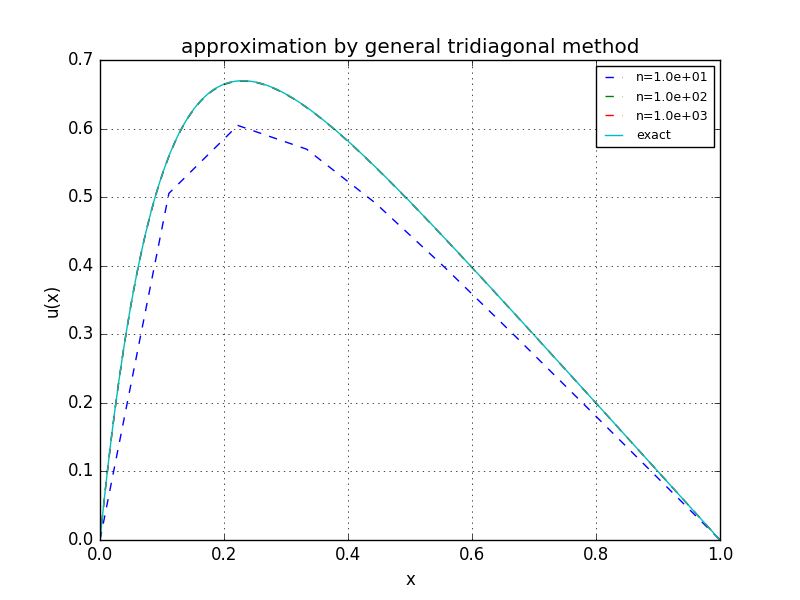
\includegraphics[scale=0.7]{../img/compare_general_exact.png}
		\caption{Compare calculated u(x) with exact solution of u(x) for three values of n, using the general tridiagonal solver.}
		\label{fig:compare_gen_exact}
	\end{figure}

\subsection{CPU-time}
\begin{table}[H]
		\label{table:cpu-time}
		\begin{tabular}{|c|c|c|c|} \hline
			$\log_{10}(n)$ & general tridiagonal[s] & specific tridiagonal[s] & LU decomposition [s] \\ \hline
			1 & 0.000010 & 0.000006 & 0.008585 \\
			2 & 0.000047 & 0.000007 & 0.015610 \\
			3 & 0.000159 & 0.000123 & 0.699342 \\
			4 & 0.001421 & 0.001749 & \\
			5 & 0.020054 & 0.024508 & \\
			6 & 0.056499 & 0.064189 & \\ \hline
		\end{tabular}
		\caption{CPU-time each methods use for calculating u(x) in seconds.}
	%\end{table}
	%\begin{table}[h!]
		\label{table:cpu-frequency}
		\begin{tabular}{|c|c|c|c|} \hline
			$\log_{10}(n)$ & general tridiagonal[s] & specific tridiagonal[s] & LU decomposition [s] \\ \hline
			1 & 1e+6 & 1.67e+6 & 1.16e+3 \\
			2 & 2.13e+6 & 1.43e+7 & 6.40e+3 \\
			3 & 6.29e+6 & 8.13e+6 & 1.43e+3 \\
			4 & 7.03e+6 & 5.72e+6 & \\
			5 & 4.99e+6 & 4.08e+6 & \\
			6 & 1.77e+7 & 1.56e+7 & \\ \hline
		\end{tabular}
		\caption{Matrix size per computation time. This data was found by dividing n (in table \hyperref[table:cpu-time]{table 1} by computational time in the same table).}
	%\end{table}
	%\begin{table}[h!]
		\label{table:flops-per-sec}
		\begin{tabular}{|c|c|c|c|} \hline
			$\log_{10}(n)$ & general tridiagonal[s] & specific tridiagonal[s] & LU decomposition [s] \\ \hline
			1 & 9e+6 & 6.68e+6 & x $\times$ 1.16e+3 \\
			2 & 1.92e+7 & 5.72e+7 & x $\times$ 6.4e+3 \\
			3 & 5.66e+7 & 3.25e+7 & x $\times$ 1.43e+3 \\
			4 & 6.33e+7 & 2.29e+7 & \\
			5 & 4.49e+7 & 1.63e+7 & \\
			6 & 1.59e+8 & 6.24e+7 & \\ \hline
		\end{tabular}
		\caption{Flops per second where found by multiplying table \ref{table:cpu-frequency} by the number of flops per iteration (9 for general and 4 for specific)}
\end{table}
	
\subsection{Relative error}
	\begin{table}[H]
	\centering
		\label{table:relerror}
		\begin{tabular}{|c|c|c|} \hline
			n & $\log_{10}(h)$ & $\epsilon$ \\
			10 & -1.0414 & -1.0140 \\
			100 & -2.0043 & -3.0709 \\	
			1000 & -3.0004 & -5.0381 \\
			10000 & -4.0000 & -3.9641 \\ \hline
		\end{tabular}
		\caption{table of epsilon-values of various step-lengths}
	\end{table}
	\begin{figure}[H]
		\label{fig:relerror}
		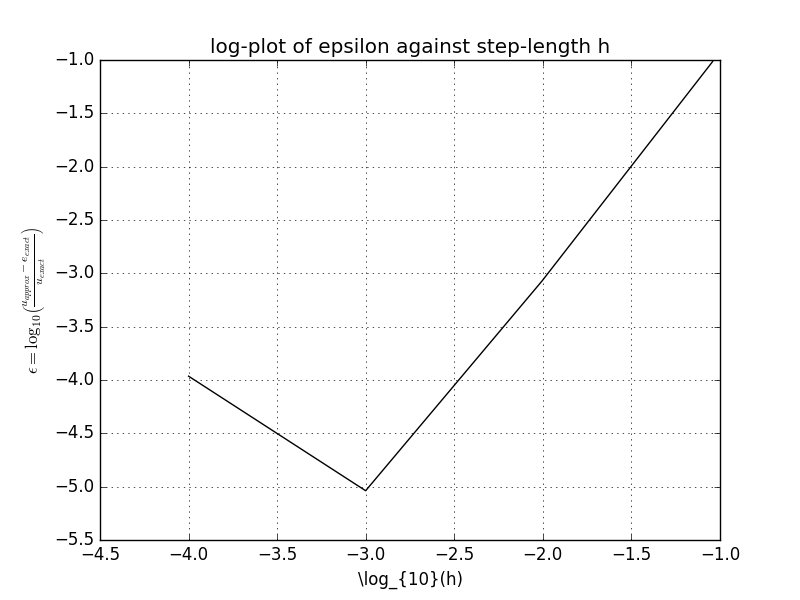
\includegraphics[scale=0.7]{../img/epsilon.png}
		\caption{log-log-plot of table \ref{table:rel_error}}
	\end{figure}
	
\section{Conclusion and discussion}
From \hyperref[section:results]{section 4} it becomes clear that the numerical solvers are quite accurate for n=100 and above(h=1/99 and below). This becomes clear when one examines figure \hyperref[fig:compare_gen_exact]{figure 3} where the approximation by solver lies on top of the exact solution for n=10 and n=100.
	
When it comes to computing time, the LU-decomposition is much less efficient(to no surprise for anyone), however there seems to be a slight bug in the timing of specific tridiagonal solver. This method becomes $slower$ than the general solver for high values of n, as opposed to the previous expectation (recall that the specific algorithm calculates by $\simeq$ 4n flops, while the general, algebraic algorithm calculates by $\simeq$ 9n flops).
	
By looking at \hyperref[table:flops-per-sec]{table 2} the number of total floating point operations per second should the same for all three methods since they are all run on the same computer, however there are discrepencies when comparing the specific and general solvers, as mentioned earlier. the number of floating point operations per iteration for the LU-decomposition can now be determined by solving for x. This factor x is 7758, 3000 and 39580 for the three recorded instances of LU-decomposition. The results are way away of from eachother (hinting towards errors in the program CPU-timing or calculation), but they are all very much larger than the factors 9 and 4 in the general and specific methods.

The program was unsuccesful at storing the data for values of n larger then 1e+4, so the graph of epsilon streches over a limited span of values, however a trend still appears. As the step-length decreases the relative error also decreases (with a slope of $\epsilon = h^2$), until it hits a minimum value at $h=10^{-3}$ and starts increasing with a slope of $\epsilon = -h$ as h decreases further.

\section{Appendix - Github}
\label{section:github}

\end{document}
